\documentclass{article}[12pt]
\usepackage{fullpage}
\usepackage[ruled,lined,linesnumbered]{algorithm2e}
\usepackage{algpseudocode}
\usepackage{multicol}
\usepackage{amsmath}
\usepackage{amsfonts}
\usepackage{amsthm}
\usepackage{amssymb}
\usepackage{enumitem}
\usepackage{url}
\usepackage{graphicx}
\usepackage{float}

\begin{document}
{\centering\section*{Project3 Report}}
\begin{center}
	Zhuocheng Shang 862188698 and Zizhuo Wang 862325178
\end{center}
\section{Algorithm}
\begin{algorithm}[H]
	\caption{Compute }\label{algo:algo}
	VARKILL(N) = $\emptyset$ \\
	UEVar(N) = $\emptyset$ \\
	FOR i = 1 to k \\
	\qquad assume $i_{i}$ is x $\leftarrow$ y op z\\
	\qquad IF y $\notin $ VARKILL(N) \\
	\qquad\qquad UEVar(N) = UEVAR(N) $\cup $ y\\
\qquad 	IF z $\notin $ VARKILL(N)\\
	\qquad\qquad UEVar(N) = UEVAR(N) $\cup $ z\\
	\qquad VARKILL(N) = VARKILL(N) $\cup $ x\\
\end{algorithm}

\begin{algorithm}[H]
	\caption{Iterative}
	FOR block N in CFG \\
	\qquad LIVEOUT(N) = $\emptyset$\\UEVar and Varkill
	\qquad \textit{continue} = true\\
	WHILE(\textit{continue})\\
	\qquad \textit{continue} = false\\
	\qquad FOR block N in CFG\\
	\qquad \qquad LIVEOUT(N) = $ \cup_{X \in SUCC(N)}$  (LIVEOUT(X)-VARKILL(X) $\cup$ UEVar(X))\\
	\qquad \qquad IF LIVEOUT(N) changed\\
	\qquad\qquad\qquad \textit{continue} = true
\end{algorithm}
\section{Data structures}

There are three major map structures that are used:  UEVAR\underline{~}table,VARKILL\underline{~}table and  LIVEOUT\underline{~}table. In each table, the keys are the names of the basic blocks and the values are the UEVar sets, the VARkill sets or the Liveout sets of the corresponding basic blocks.
\section{Implementation details}
First, we compute UEVar and Varkill for each basic block. If an instruction is a load instruction, then we add the operand to UEVar. If an instruction is a store instruction, then we add the operand to Varkill. 

\begin{figure}[H]
	\centering
	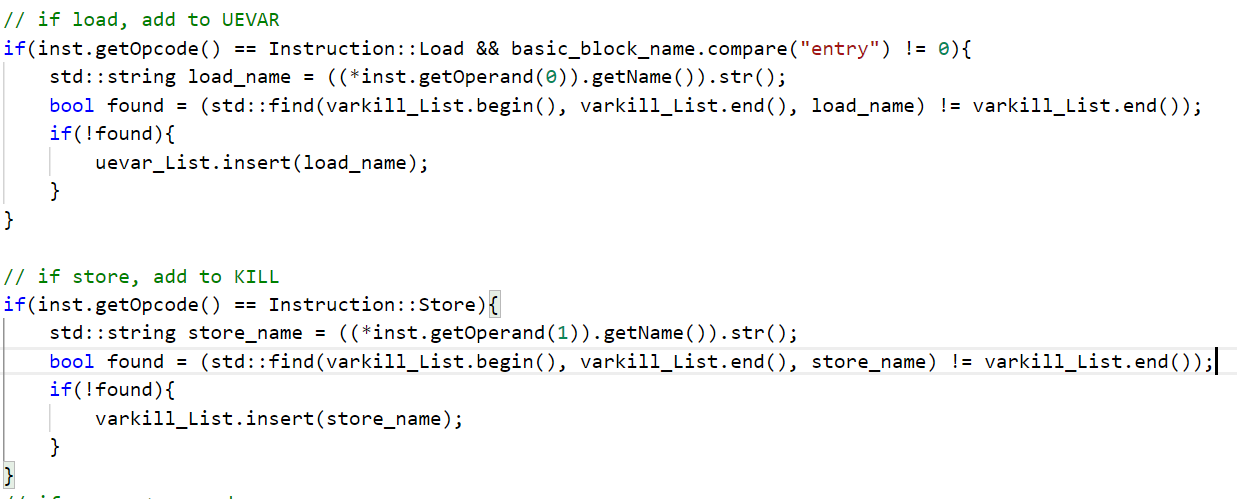
\includegraphics[width=0.7\linewidth]{1}
\end{figure}
\\\\
If an instruction is a computing instruction, we firsr check if the operands is a constant. If not, check if they are in the Varkill list. If they are also not in it, we will add them into the UEVar list.
\begin{figure}[H]
	\centering
	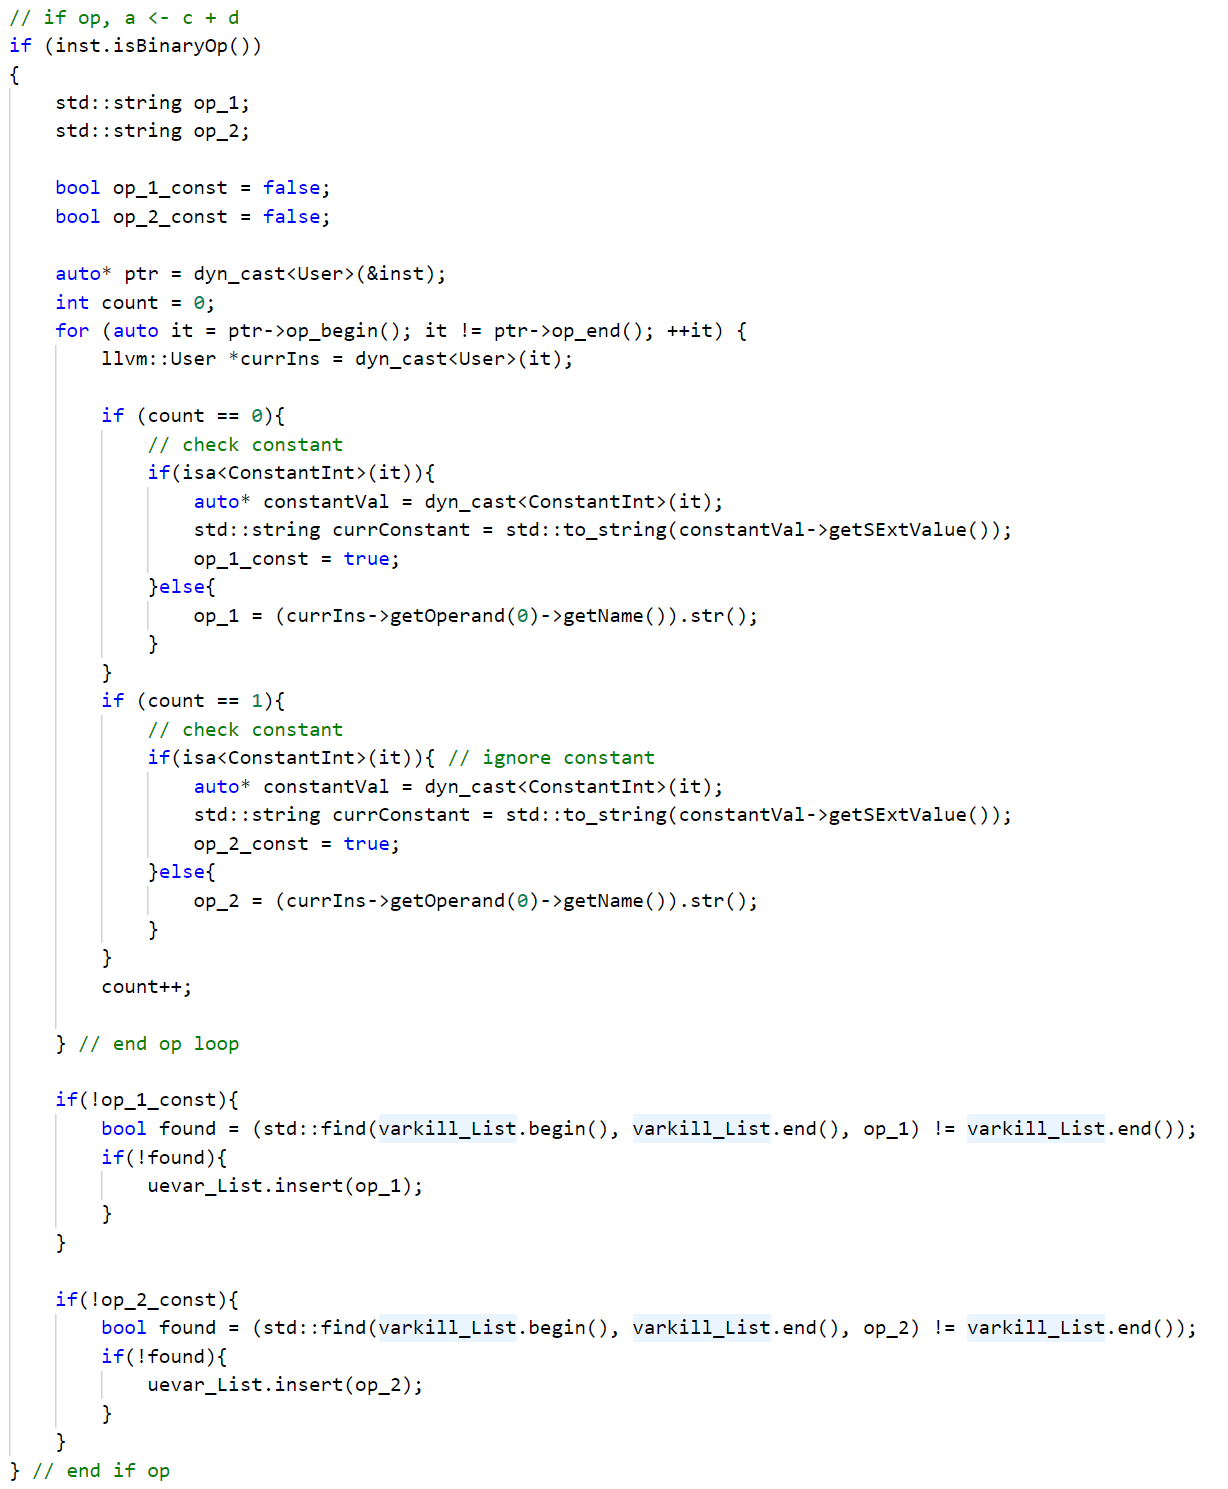
\includegraphics[width=0.7\linewidth]{2}
\end{figure}
\newpage
After finding the UEVar and Varkill for all the basic blocks, we compute the liveout sets for each basic block using iteration. In each round, we update the liveout sets for each basic block with the formula LIVEOUT(N) = $ \cup_{X \in SUCC(N)}$  (LIVEOUT(X)-VARKILL(X) $\cup$ UEVar(X)). When the liveout sets of each basic block no longer change, the iteration stops.
\begin{figure}[H]
	\centering
	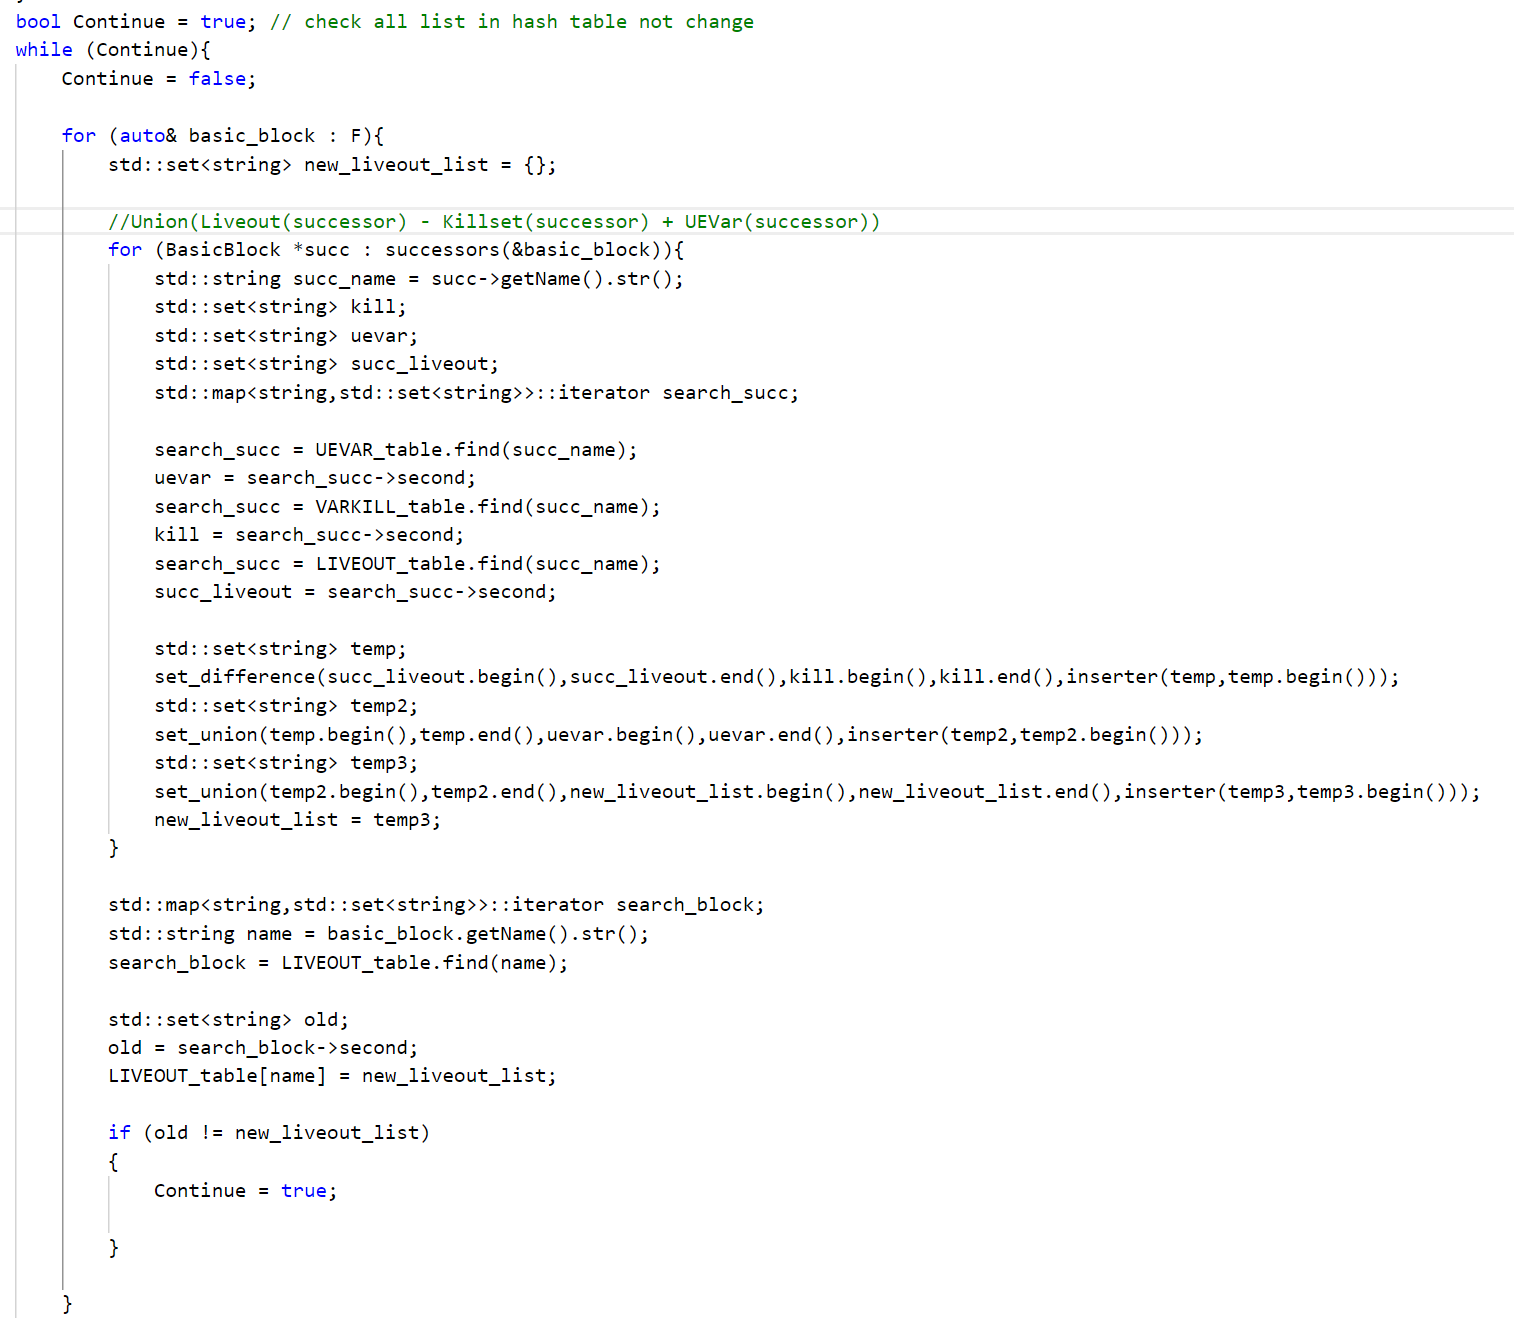
\includegraphics[width=0.7\linewidth]{3}
\end{figure}
\\\\
Finally, we output the result of each basic block one by one.
\begin{figure}[H]
	\centering
	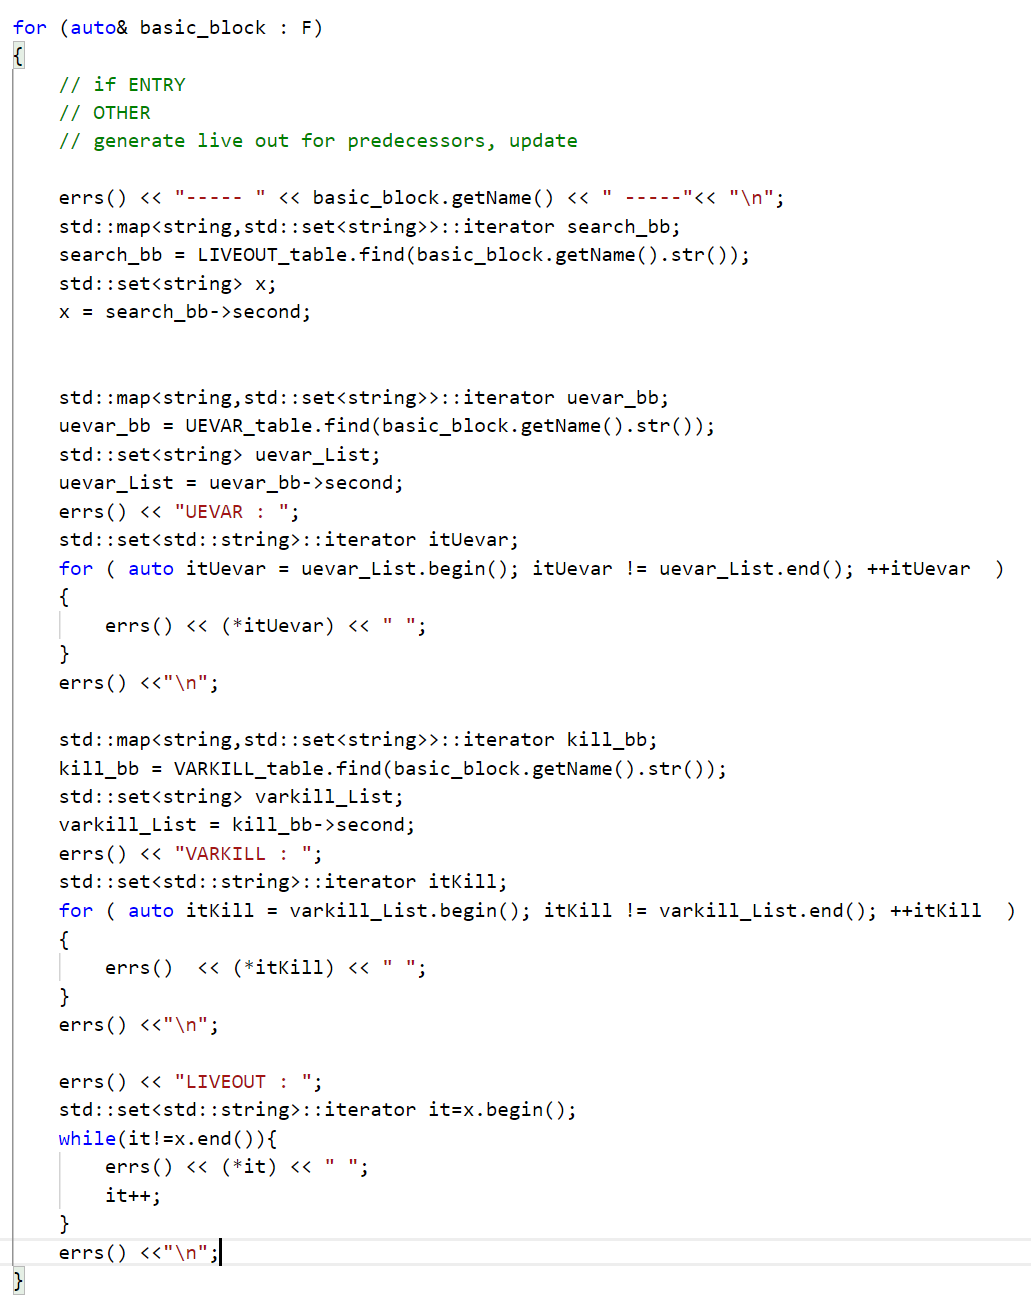
\includegraphics[width=0.7\linewidth]{4}
\end{figure}

\end{document}

